%! TEX root = main.tex
\documentclass[czech,maturita,a4paper,bachelor]{diploma}

%todo notes setup 
\usepackage[colorinlistoftodos,prependcaption,textsize=tiny]{todonotes}
\definecolor{Plum}{RGB}{255,87,51}
\usepackage[utf8]{inputenc}
% \usepackage{graphicx} % Required for inserting images
% %bibilography setup

% %czech language setup
 % \usepackage[czech]{babel}
% Packages
\usepackage{float}
\usepackage{fvextra}
\usepackage[autostyle=true,czech=quotes]{csquotes} % korektni sazba uvozovek, podpora pro balik biblatex
\usepackage[backend=biber, style=iso-numeric, alldates=iso,
sorting=ynt,
bibencoding=utf8,
sortlocale=cs-CZ %sorts according to czech alphabet
]{biblatex} % bibliografie
\usepackage{dcolumn} % sloupce tabulky s ciselnymi hodnotami
\usepackage{subfig} % makra pro "podobrazky" a "podtabulky"
\usepackage[php]{diplomalst}



\usepackage{xargs}% Use more than one optional parameter in a new commands
\usepackage[rgb, hyperref]{xcolor}  % Coloured text etc.

\usepackage{minted}
\usepackage{tcolorbox}
\usepackage{etoolbox}

\usepackage{pgf-pie}


% Hyphenate in texttt
\usepackage[htt]{hyphenat}

%allows including of external tex files
%used to include sections
\usepackage{subfiles}


\newcommandx{\unsure}[2][1=]{\todo[disable,linecolor=red,backgroundcolor=red!25,bordercolor=red,#1]{#2}}
\newcommandx{\change}[2][1=]{\todo[disable,linecolor=blue,backgroundcolor=blue!25,bordercolor=blue,#1]{#2}}
\newcommandx{\info}[2][1=]{\todo[disable,linecolor=OliveGreen,backgroundcolor=OliveGreen!25,bordercolor=OliveGreen,#1]{#2}}
\newcommandx{\improvement}[2][1=]{\todo[disable,linecolor=Plum,backgroundcolor=Plum!25,bordercolor=Plum,#1]{#2}}
\newcommandx{\thiswillnotshow}[2][1=]{\todo[disable,#1]{#2}}


\addbibresource{references.bib} %Import the bibliography file


\definecolor{graph1}{RGB}{185, 163, 148}
\definecolor{graph2}{RGB}{237, 240, 96}
\definecolor{graph3}{RGB}{240, 128, 60}
\definecolor{graph4}{RGB}{199, 239, 207}







% needs LuaTex
% \babelprovide[transforms = hyphen.repeat]{czech}





%custom command to display code names
\newcommand{\codename}[1]{\texttt{#1}}


%custom command to cross reference with viz
\newcommand{\vizref}[1]{(viz \ref{#1})}

\newenvironment{code}[1][h]{
  \begin{listing}[#1]
  \captionsetup{type=listing}
}
{
  \end{listing}  
}

\newtcolorbox{mybox}{colback=white, colframe=black} 


\BeforeBeginEnvironment{minted}{\begin{mybox}}%
\AfterEndEnvironment{minted}{\end{mybox}}%

% Parameters
\ThesisAuthor{Marek Konrád}
\ThesisSupervisor{RNDr. Rostislav Miarka, Ph.D.}
\CzechThesisTitle{Vizeval: Evaluační nástroj výuky}
\EnglishThesisTitle{Vizeval: Evaluation Tool for Education}
\StudyProgram{Informační technologie}
\SubmissionYear{2023/2024}
\ThesisAssignmentFileName{zadani.pdf}


%acronyms explained here
\AddAcronym{XML}{Extensible Markup Language}
\AddAcronym{PHP}{PHP: Hypertext Preprocessor}
\AddAcronym{MVC}{Model View Controller}
\AddAcronym{ORM}{Object Relational Mapping}
\AddAcronym{CRUD}{Create Read Update Delete}
\AddAcronym{SQL}{Structured query language}
\AddAcronym{DQL}{Doctrine Query Language}
\AddAcronym{HTML}{HyperText Markup Language}
\AddAcronym{SPA}{Single-page application}
\AddAcronym{XSRF}{Cross-site request forgery}
\AddAcronym{UX}{User experience}
\AddAcronym{ER}{Entity–relationship}
\AddAcronym{CSV}{Comma-separated values}
\AddAcronym{XLS}{Excel Binary File Format}

\CzechAbstract{
\improvement{improve abstract to catch readers attention}
Tato práce se zabývá import částí evaluačního nástroje, který vynikl jako týmová dlouhodobá maturitní práce.
Cílem bylo udělat efektivní nástroj pro hodnocení kvality výkuky a poskytnutí přehledných výsledků vedení školy a učitelům.
Dosahuje toho pomocí anket kde respondenti hodnotí daný úvazek.
Tento nástroj je realizován formou webové aplikace využívající moderní PHP.
Jeho primární účel je poskytnutí zpětné vazby pedagogům a vedení školy.
Je koncipován pro prostředí středních škol.
}
\CzechKeywords{Autoevaluace; Škola; Webová aplikace; Symfony; PHP }
\EnglishAbstract{
This document describes import functionality of the evaluation tool. The evaluation tool was created as a team long-term school ending exam. 
The goal was to make an effective evaluation tool for rating the quality of education and to provide well structured results for school management and teachers.
It is achieved by creating questionnaires about the lessons. The tool is implemented in the form of a web application using modern PHP.
The primary use case is to provide feedback to teachers and school management.
It is conceived for use in secondary schools.
}

\EnglishKeywords{Self-evaluation; School; Web application; Symfony; PHP}


\Acknowledgement{Rád bych poděkoval Davidovi Moškořovi a Honzovi Radovi za spolupráci na tomto projektu. Děkuji panu učiteli Miarkovi za vedení práce. A v neposlední řadě děkuji vedení školy za možnost testovacího nasazení. }


\begin{document}


\MakeTitlePages
\chapter{Úvod}
\subfile{sections/uvod/motivace.tex}
\subfile{sections/uvod/cile.tex}
\subfile{sections/uvod/podobne-projekty.tex}


\chapter{Tvorba aplikace}
\subfile{sections/uvod/pouzite-technologie.tex}
\subfile{sections/postup}


% \chapter{Uživatelský manuál}
% formou přílohy ?

\chapter{Závěr}
\subfile{sections/zaver.tex}
\printbibliography[title={Literatura}]


\addcontentsline{toc}{chapter}{Přílohy}
\appendix

% \documentclass[maturita, czech]{diploma}
% \usepackage{graphicx} % Required for inserting images
% \usepackage{float}
% % \usepackage[czech]{babel}
%
% % \title{manual}
% % \author{konrad.marek }
% % \date{April 2024}
%
%
%
%
%
% \begin{document}
%

\chapter{Uživatelský manuál}

Import naleznete v administraci v boční záložce. 


\section{Import ze školního systému}
V tomto kroku je důležité zvolit správný typ importu.

Tiskové sestavy vygenerujte pomocí rozhraní Bakalářů. Jedná se o sestavy:
\begin{itemize}
    \item \textbf{Seznam předmětů} dle abecedy
    \item \textbf{Úvazky} učitelů s výčtem studentů
    \item \textbf{Seznam skupin} - u všech skupin výčet po řádcích
\end{itemize}
Sestavy nahrajte.

V případě XML importu vyberte vygenerovaný XML soubor.
\begin{figure}[H]
    \centering
    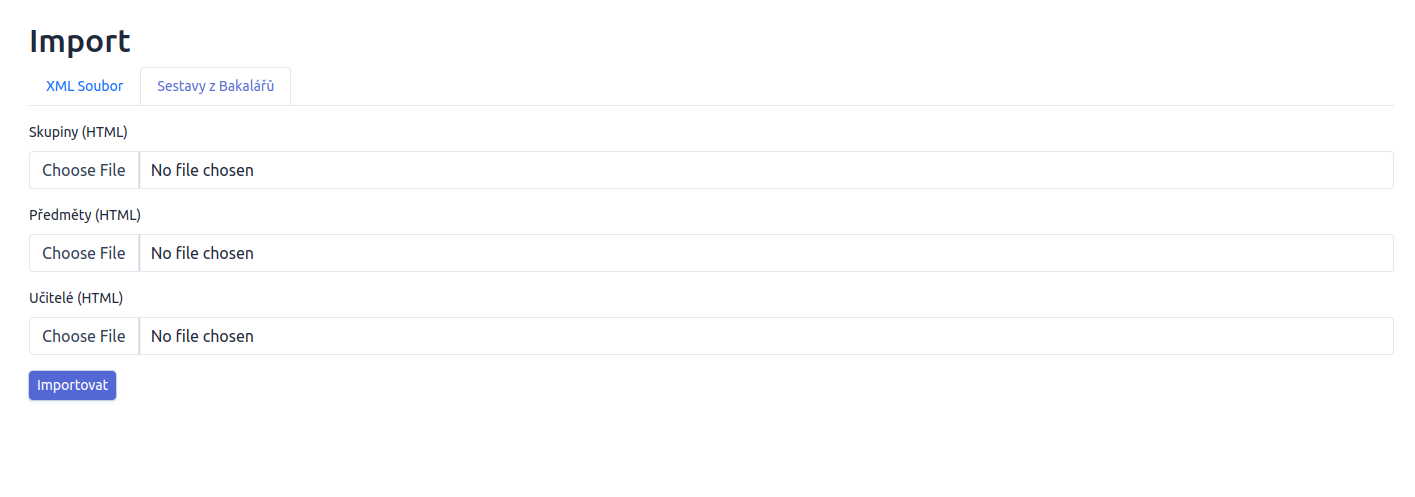
\includegraphics[width=1\linewidth]{Figures/uvodni_import.png}
    \caption{Nahrání sestavy}
    \label{fig:uvodni-import}
\end{figure}
\newpage
\section{Informace o importu}
Tento krok pouze zobrazuje informace o importu ze školního systému.
\begin{figure}[H]
    \centering
    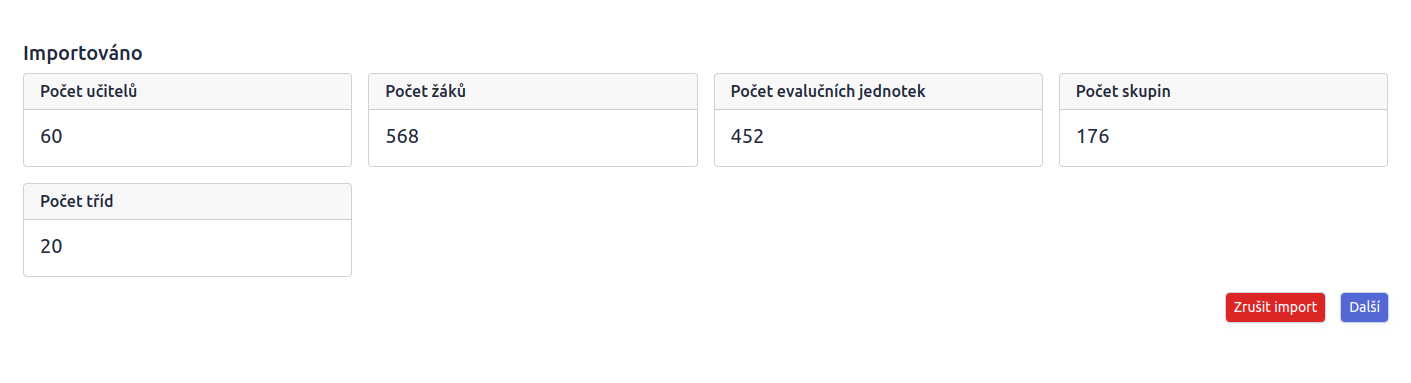
\includegraphics[width=1\linewidth]{Figures/statistika.png}
    \caption{Ukázka informací o importu}
    \label{fig:informace}
\end{figure}

\section{Spojování skupin}
Tento krok je pouze pro import ze sestav.

Jedná se o spojení skupin složených z více tříd. Vyberte kombinaci učitel-předmět a přiřaďte jim skupiny, které se učí spolu. Tlačítkem přidat skupinu naklonujete kombinaci učitel-předmět. Opakujte tento postup dokud nebudete mít vše přiřazeno. Tento krok je nutný, aby úvazky, které jsou učeny zvlášť měly také zvlášť hodnocení.

\begin{figure}[H]
    \centering
    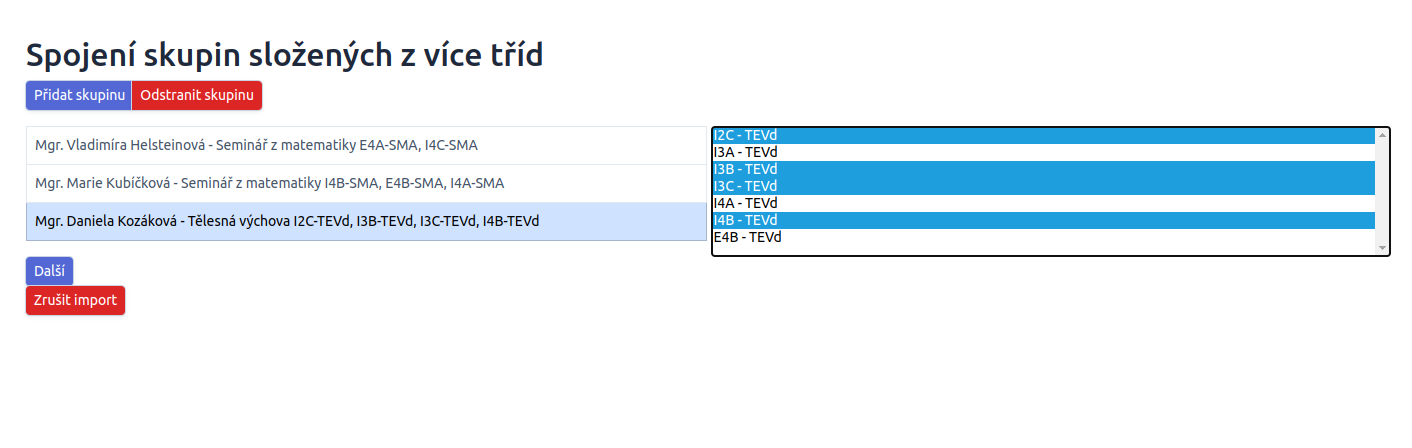
\includegraphics[width=1\linewidth]{Figures/spojovani-skupin.png}
    \caption{Ukázka spojování skupin}
    \label{fig:spojování-skupin}
\end{figure}

\section{Generování emailů}
Pokud nemáte ve školním systému školní emaily žáků bude nutný tento krok. Podobně vypadající krok je i pro generování učitelských emailů. Pro generování emailů se řiďte pokyny aplikace.

\begin{figure}[H]
    \centering
    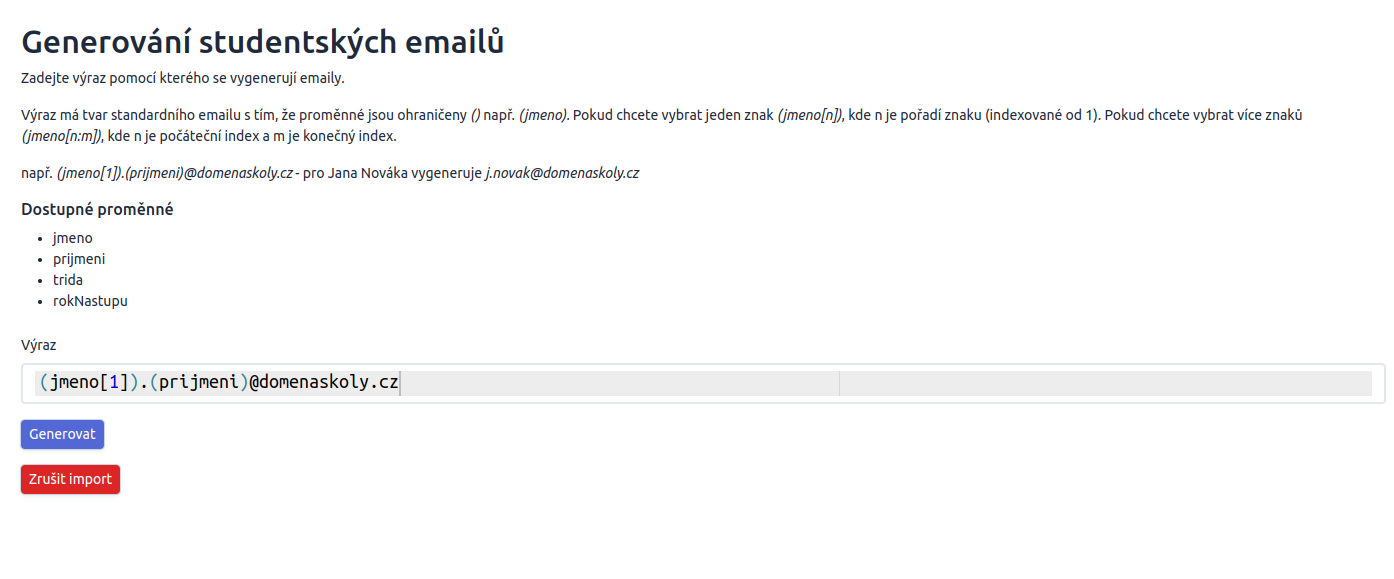
\includegraphics[width=1\linewidth]{Figures/generovani-emailu.png}
    \caption{Ukázka generování emailů}
    \label{fig:generovani-emailu}
\end{figure}


\section{Úprava duplikátních emailů}
Při generování emailů mohlo dojít k vytvoření duplikátů. V tomto kroku se duplikáty odstraní. Ručně přepište emaily žáků.

\begin{figure}[H]
    \centering
    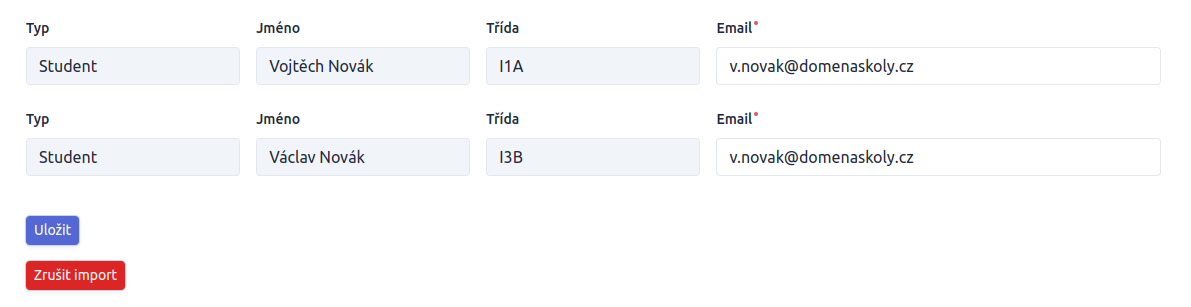
\includegraphics[width=1\linewidth]{Figures/deduplikace.png}
    \caption{Ukázka úpravy duplikátních emailů}
    \label{fig:deduplikace}
\end{figure}


% \end{document}



\end{document}
